\documentclass{article}
\usepackage{xcolor}
\usepackage{titleps}
\usepackage[letterpaper, margin=0.95in]{geometry}
\usepackage{url}
\usepackage{amsmath}
\usepackage{amssymb}
\usepackage{wrapfig}
\usepackage{float}
\usepackage{mathtools}
\usepackage{enumitem}
\usepackage{tabu}
\usepackage{parskip}
\usepackage{natbib}
\usepackage{listings}

\usepackage[many]{tcolorbox}
\usepackage{minted}
\setminted[python]{
	% frame=single,
	% linenos,
    xleftmargin=0.475em,
    baselinestretch=1.2,
}
% https://tex.stackexchange.com/a/569249
\setcounter{secnumdepth}{5}
\setcounter{tocdepth}{5}
\makeatletter
\newcommand\subsubsubsection{\@startsection{paragraph}{4}{\z@}{-2.5ex\@plus -1ex \@minus -.25ex}{1.25ex \@plus .25ex}{\normalfont\normalsize\bfseries}}
\newcommand\subsubsubsubsection{\@startsection{subparagraph}{5}{\z@}{-2.5ex\@plus -1ex \@minus -.25ex}{1.25ex \@plus .25ex}{\normalfont\normalsize\bfseries}}
\makeatother

\usepackage{hyperref}
\usepackage[color=red]{todonotes}
\usepackage{forest}
\definecolor{light-yellow}{HTML}{FFE5CC}

\newpagestyle{ruled}
{\sethead{CMU 16-831}{Introduction to Robot Learning }{Spring 2024}\headrule
  \setfoot{}{}{}}
\pagestyle{ruled}

\renewcommand\makeheadrule{\color{black}\rule[-.75\baselineskip]{\linewidth}{0.4pt}}
\renewcommand*\footnoterule{}

\newtcolorbox[]{answer}[1][]{
    % breakable,
    enhanced,
    nobeforeafter,
    colback=white,
    title=Your Answer,
    sidebyside align=top,
    box align=top,
    #1
}



\begin{document}

\lstset{basicstyle = \ttfamily,columns=fullflexible,
backgroundcolor = \color{light-yellow}
}

\begin{centering}
    {\Large Assignment 2: Policy Gradient} \\
    \vspace{.25cm}
    % \textbf{Due September 13, 11:59 pm} \\
\end{centering}
\vspace{0.25cm}

\textbf{Andrew ID:} \texttt{jihyunki} \\
\textbf{Collaborators:} \texttt{Write the Andrew IDs of your collaborators here (if any).}\\ 
\textbf{NOTE:} Please do \textbf{NOT} change the sizes of the answer blocks or plots.

\setcounter{section}{4}
\section{Small-Scale Experiments}

\subsection{Experiment 1 (Cartpole) -- \lbrack5 points total\rbrack}

\subsubsection{Configurations}
\begin{answer}[title=Q5.1.1,height=6cm,width=\linewidth]
\begin{minted}
[framesep=2mm, fontsize=\scriptsize, breaklines]
{bash}
python rob831/scripts/run_hw2.py --env_name CartPole-v0 -n 150 -b 1500 \
    -dsa --exp_name q1_sb_no_rtg_dsa

python rob831/scripts/run_hw2.py --env_name CartPole-v0 -n 150 -b 1500 \
    -rtg -dsa --exp_name q1_sb_rtg_dsa

python rob831/scripts/run_hw2.py --env_name CartPole-v0 -n 150 -b 1500 \
    -rtg --exp_name q1_sb_rtg_na

python rob831/scripts/run_hw2.py --env_name CartPole-v0 -n 150 -b 6000 \
    -dsa --exp_name q1_lb_no_rtg_dsa

python rob831/scripts/run_hw2.py --env_name CartPole-v0 -n 150 -b 6000 \
    -rtg -dsa --exp_name q1_lb_rtg_dsa

python rob831/scripts/run_hw2.py --env_name CartPole-v0 -n 150 -b 6000 \
    -rtg --exp_name q1_lb_rtg_na
\end{minted}
\end{answer}

\subsubsection{Plots}

\subsubsubsection{Small batch -- \lbrack1 points\rbrack}
\begin{answer}[title=Q5.1.2.1,height=9.5cm,width=\linewidth]
\centering
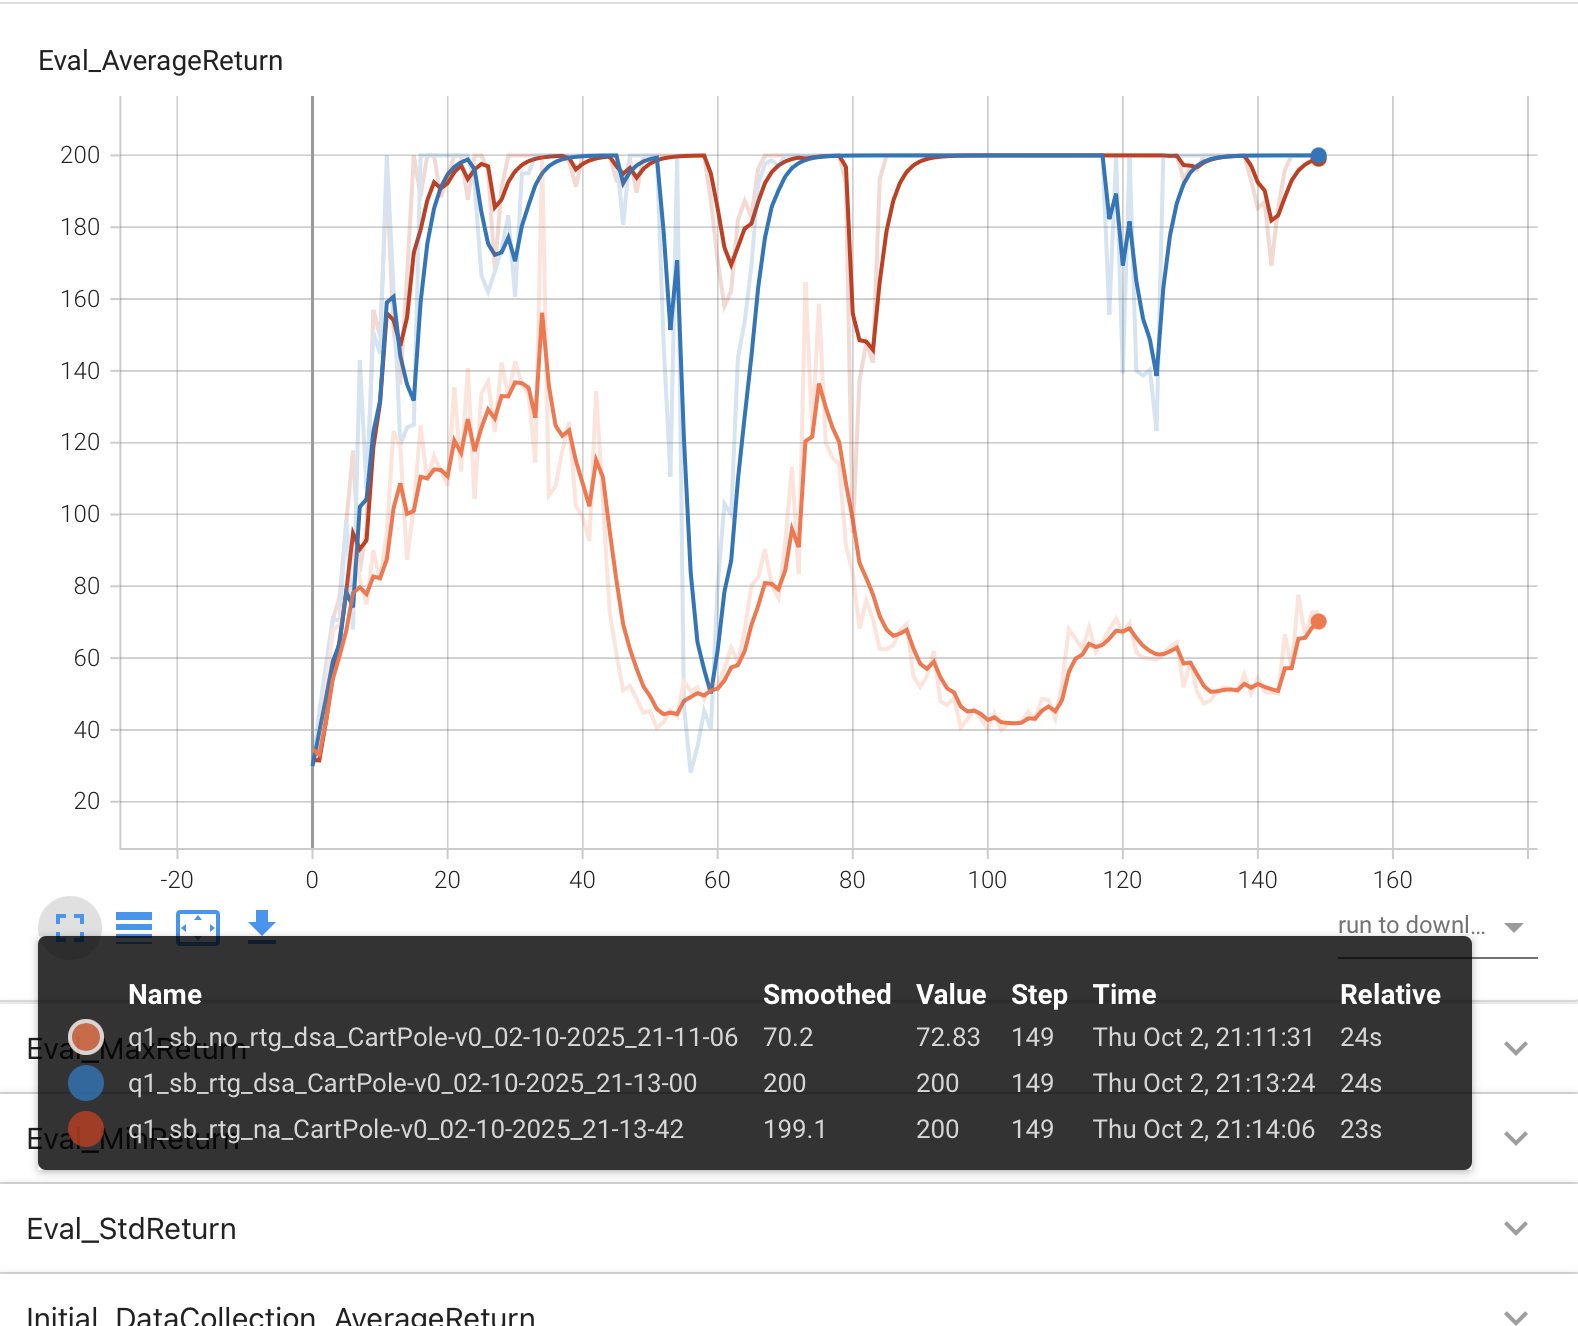
\includegraphics[height=8cm]{q1_sb.png}
\end{answer}

\subsubsubsection{Large batch -- \lbrack1 points\rbrack}
\begin{answer}[title=Q5.1.2.2,height=9.5cm,width=\linewidth]
\centering
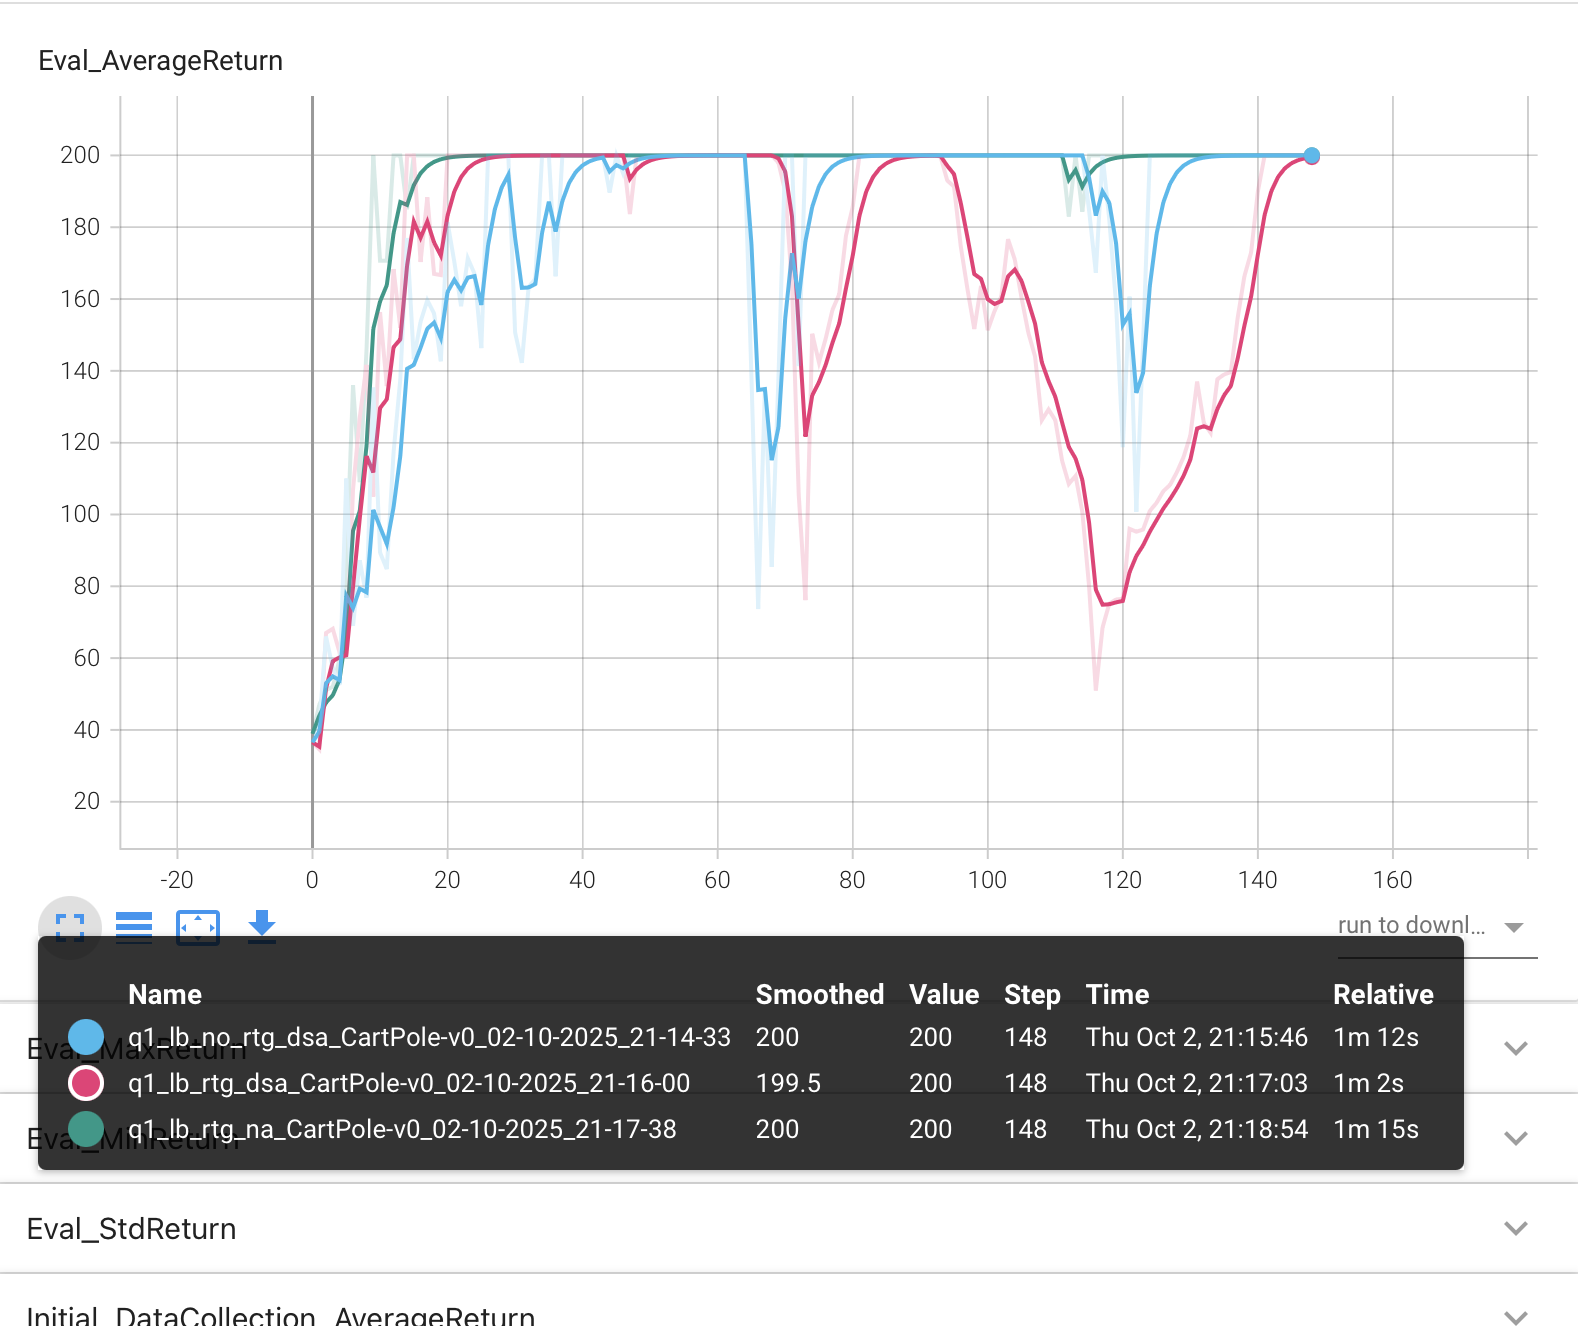
\includegraphics[height=8cm]{q1_lb.png}
\end{answer}

\subsubsection{Analysis}

\subsubsubsection{Value estimator -- \lbrack1 points\rbrack}
\begin{answer}[title=Q5.1.3.1,height=4cm,width=\linewidth]
The reward-to-go estimator shows better performance compared to the trajectory-centric estimator without advantage standardization. Across both small-batch (b=1500) and large-batch (b=6000) settings, reward-to-go policies converge more quickly to the optimal return and maintain higher stability, while trajectory-centric estimators learn more slowly and often fluctuate at lower performance. This confirms that reward-to-go provides a more informative gradient signal, enabling faster and more stable learning.
\end{answer}

\subsubsubsection{Advantage standardization -- \lbrack1 points\rbrack}
\begin{answer}[title=Q5.1.3.2,height=4cm,width=\linewidth]
Advantage standardization improves training stability across both small and large batch settings. With standardization, the learning curves become smoother and exhibit reduced variance, indicating that normalizing advantages helps stabilize updates and prevents divergence. This leads to more consistent convergence toward the optimal return.
\end{answer}

\subsubsubsection{Batch size -- \lbrack1 points\rbrack}
\begin{answer}[title=Q5.1.3.3,height=4cm,width=\linewidth]
Smaller batches lead to noisier learning curves and less consistent final returns, while larger batches provide more reliable gradient estimates and smoother convergence. Larger batch runs consistently reach higher and more stable returns, demonstrating the advantage of using greater batch sizes in this setting.
\end{answer}

\subsection{Experiment 2 (InvertedPendulum) -- \lbrack4 points total\rbrack}

\subsubsection{Configurations -- \lbrack1.5 points\rbrack}
\begin{answer}[title=Q5.2.1,height=10cm,width=\linewidth]
\begin{minted}
[framesep=2mm, fontsize=\scriptsize, breaklines]
{bash}
# Sweep used to explore b and r
for B in 800 1000 1500 2000; do
  for LR in 0.001 0.003 0.01 0.03; do
    /content/py310/bin/python -m rob831.scripts.run_hw2 \
      --env_name InvertedPendulum-v4 \
      --ep_len 1000 --discount 0.92 \
      -n 100 -l 2 -s 64 \
      -b $B -lr $LR -rtg \
      --exp_name q2_b${B}_r${LR}
  done
done

# Final chosen run (b* = 1000, r* = 0.01)
/content/py310/bin/python -m rob831.scripts.run_hw2 \
  --env_name InvertedPendulum-v4 \
  --ep_len 1000 --discount 0.92 \
  -n 100 -l 2 -s 64 \
  -b 1000 -lr 0.01 -rtg \
  --exp_name q2_b1000_r0.01
\end{minted}
\end{answer}

\subsubsection{smallest \textbf{b*} and largest \textbf{r*} (same run) -- \lbrack1.5 points\rbrack}
\begin{answer}[title=Q5.2.2,height=4cm,width=\linewidth]
The smallest batch size and largest learning rate combination that still reached the optimal score within 100 iterations was b = 1000* and r = 0.01*. This configuration converged to the maximum reward of 1000 in fewer than 100 iterations, demonstrating fast and stable learning.
\end{answer}

\subsubsection{Plot -- \lbrack1 points\rbrack}
\begin{answer}[title=Q5.2.3,height=10cm,width=\linewidth]
\centering
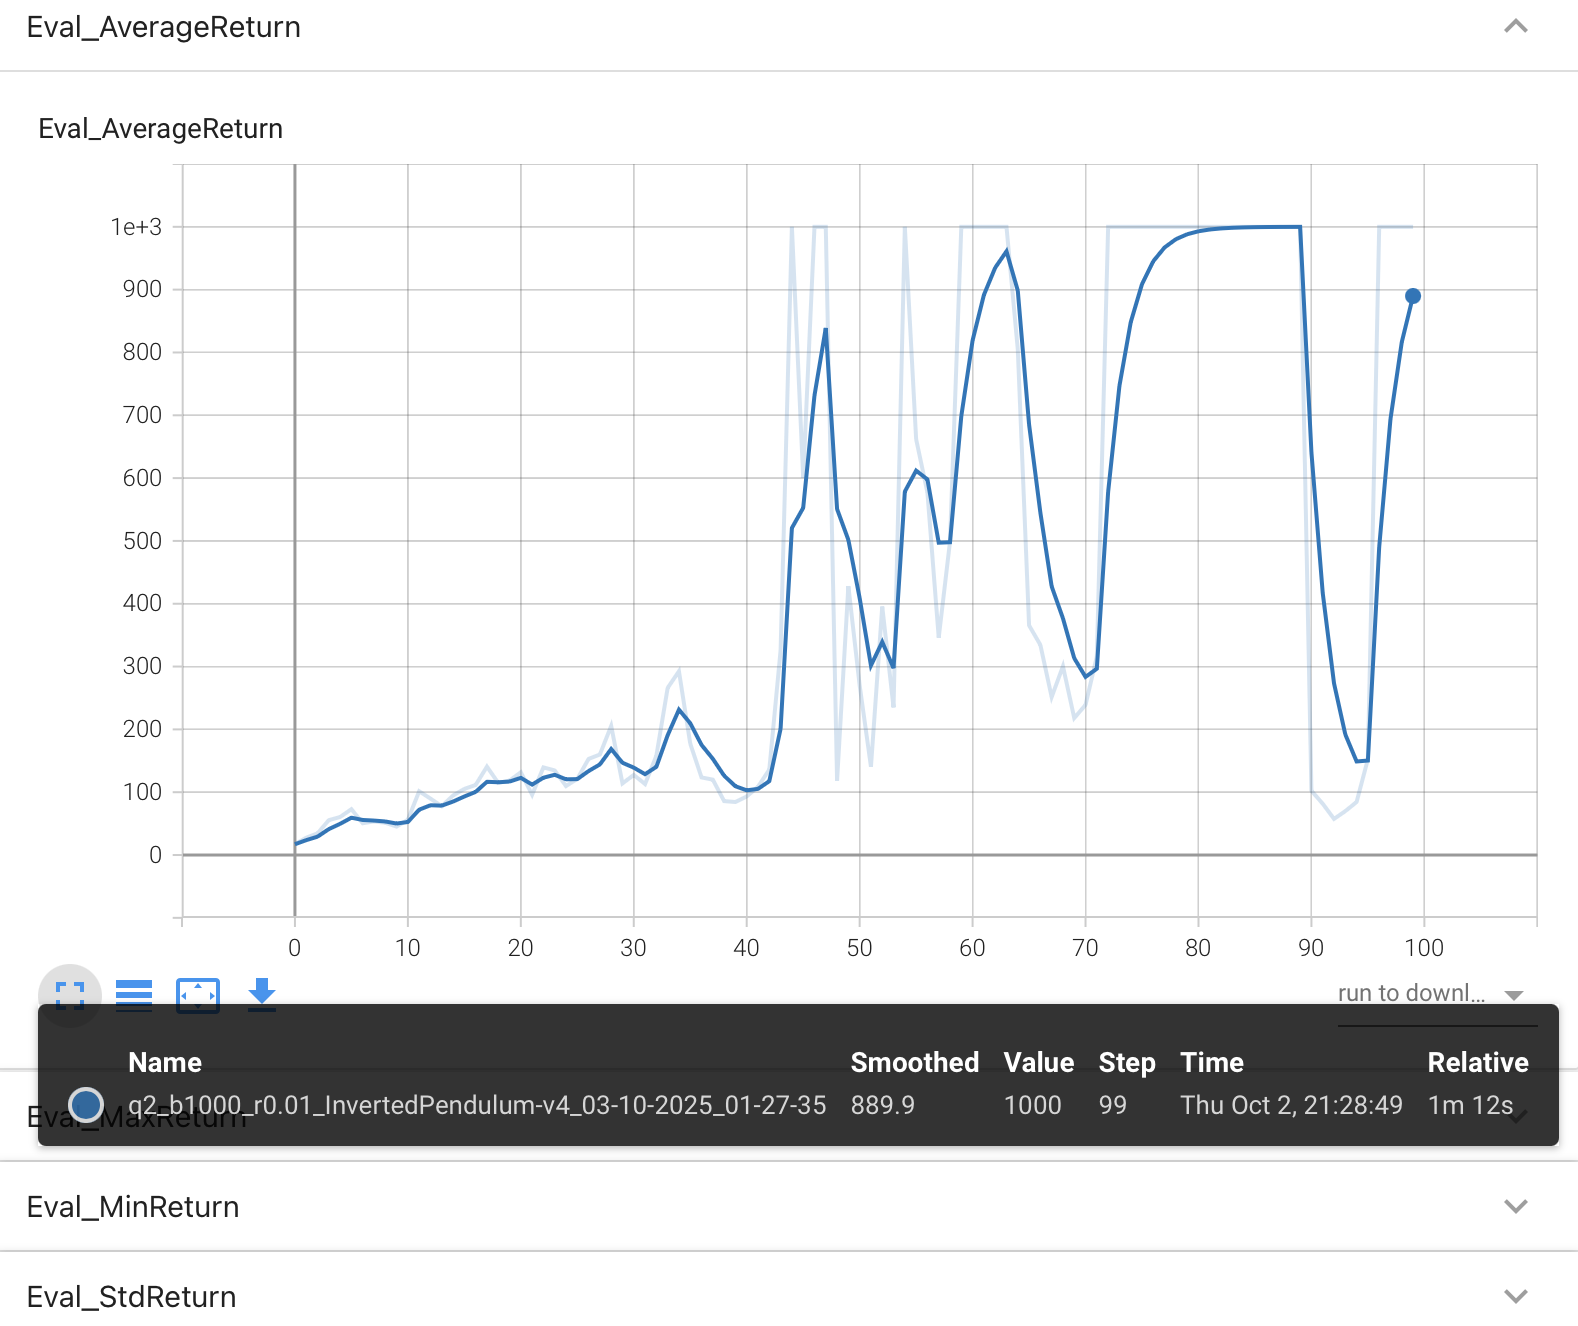
\includegraphics[height=8cm]{q2.png}
\end{answer}

\setcounter{section}{6}
\section{More Complex Experiments}

\subsection{Experiment 3 (LunarLander) -- \lbrack1 points total\rbrack}

\subsubsection{Configurations}
\begin{answer}[title=Q7.1.1,height=6cm,width=\linewidth]
\begin{minted}
[framesep=2mm, fontsize=\scriptsize, breaklines]
{bash}
python rob831/scripts/run_hw2.py \
    --env_name LunarLanderContinuous-v4 --ep_len 1000
    --discount 0.99 -n 100 -l 2 -s 64 -b 10000 -lr 0.005 \
    --reward_to_go --nn_baseline --exp_name q3_b10000_r0.005
\end{minted}
\end{answer}

\subsubsection{Plot -- \lbrack1 points\rbrack}
\begin{answer}[title=Q7.1.2,height=10cm,width=\linewidth]
\centering
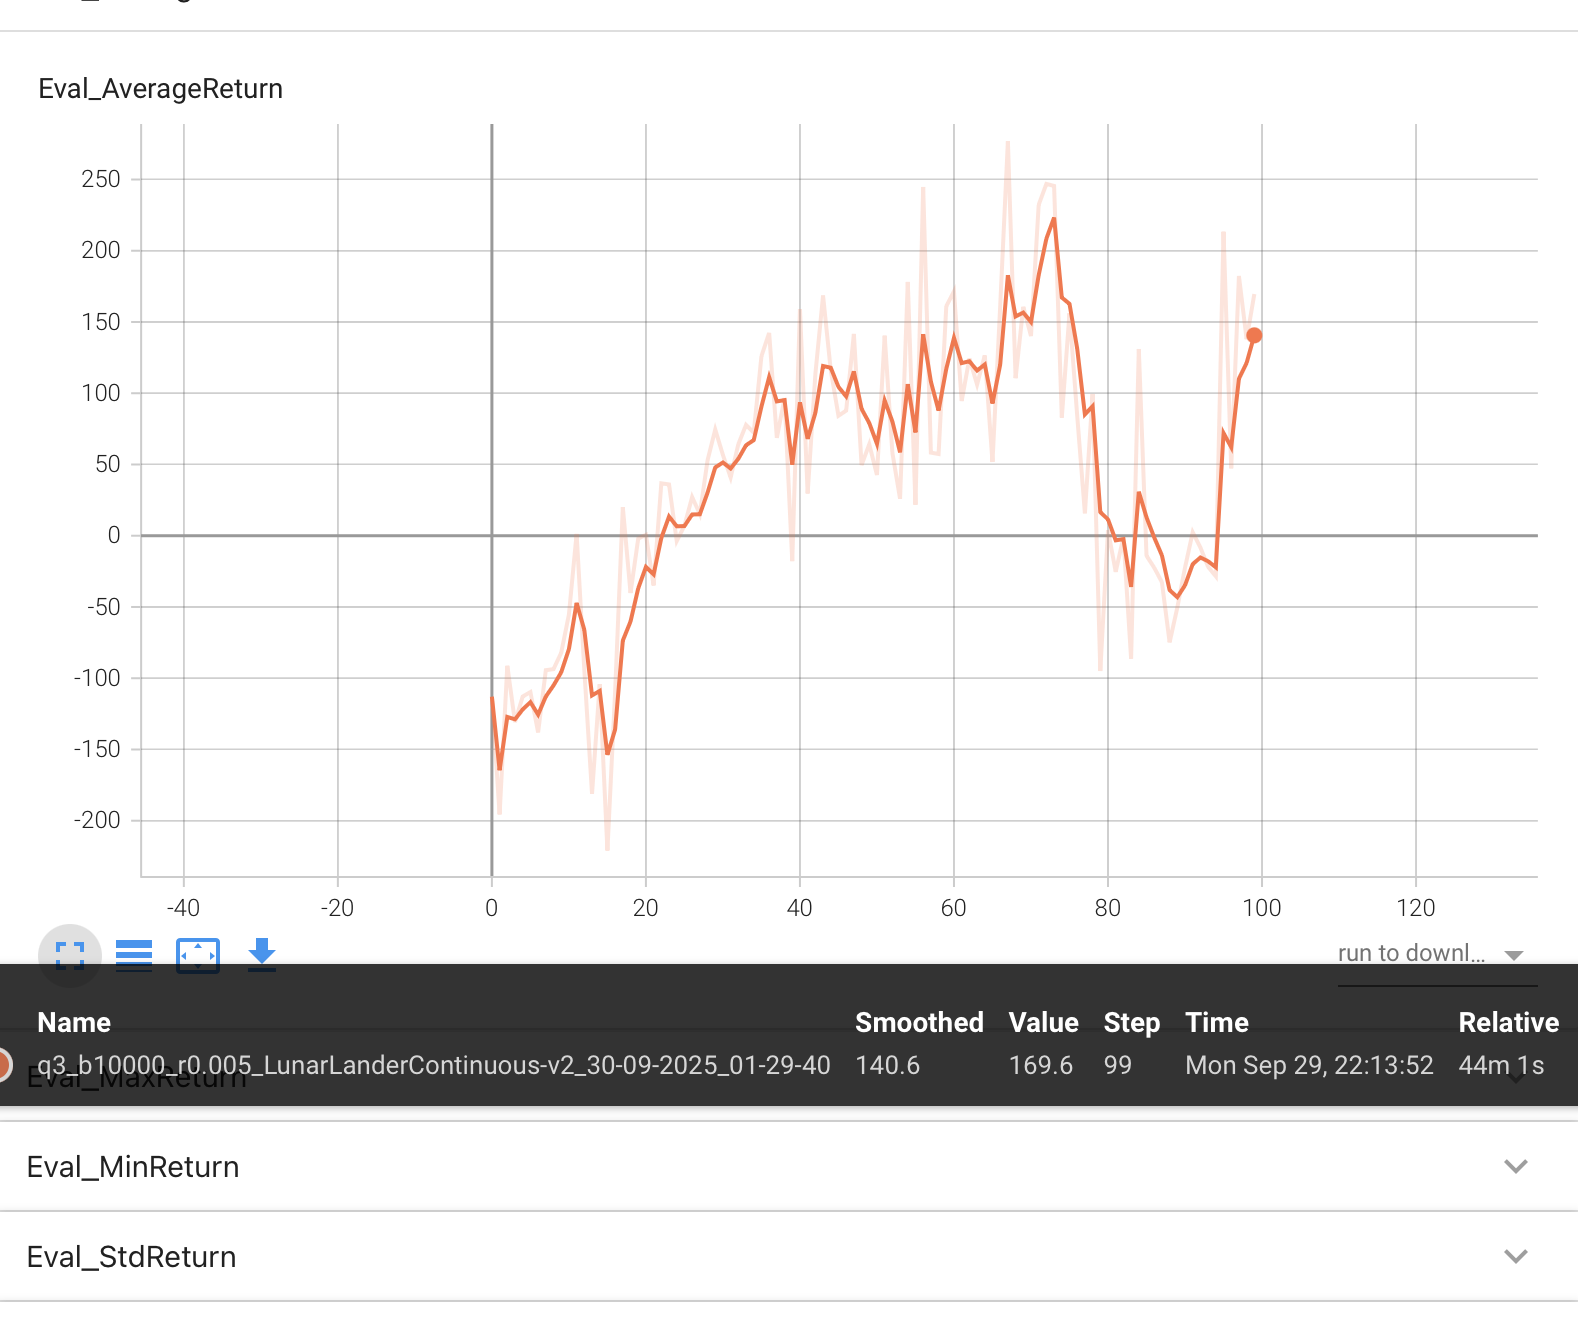
\includegraphics[height=8cm]{q3.png}
\end{answer}

\subsection{Experiment 4 (HalfCheetah) -- \lbrack1 points\rbrack}

\subsubsection{Configurations}
\begin{answer}[title=Q7.2.1,height=10cm,width=\linewidth]
\begin{minted}
[framesep=2mm, fontsize=\scriptsize, breaklines, escapeinside=||, mathescape=true]
{python}
# Search space: batch size {15000, 35000, 55000}, learning rate {0.005, 0.01, 0.02}
for B in 15000 35000 55000; do
  for LR in 0.005 0.01 0.02; do
    /content/py310/bin/python -m rob831.scripts.run_hw2 \
      --env_name HalfCheetah-v4 --ep_len 150 \
      --discount 0.95 -n 100 -l 2 -s 32 \
      -b $B -lr $LR -rtg --nn_baseline \
      --exp_name q4_search_b${B}_lr${LR}_rtg_nnbaseline
  done
done
\end{minted}
\end{answer}

\subsubsection{Plot -- \lbrack1 points\rbrack}
\begin{answer}[title=Q7.2.2,height=10cm,width=\linewidth]
\centering
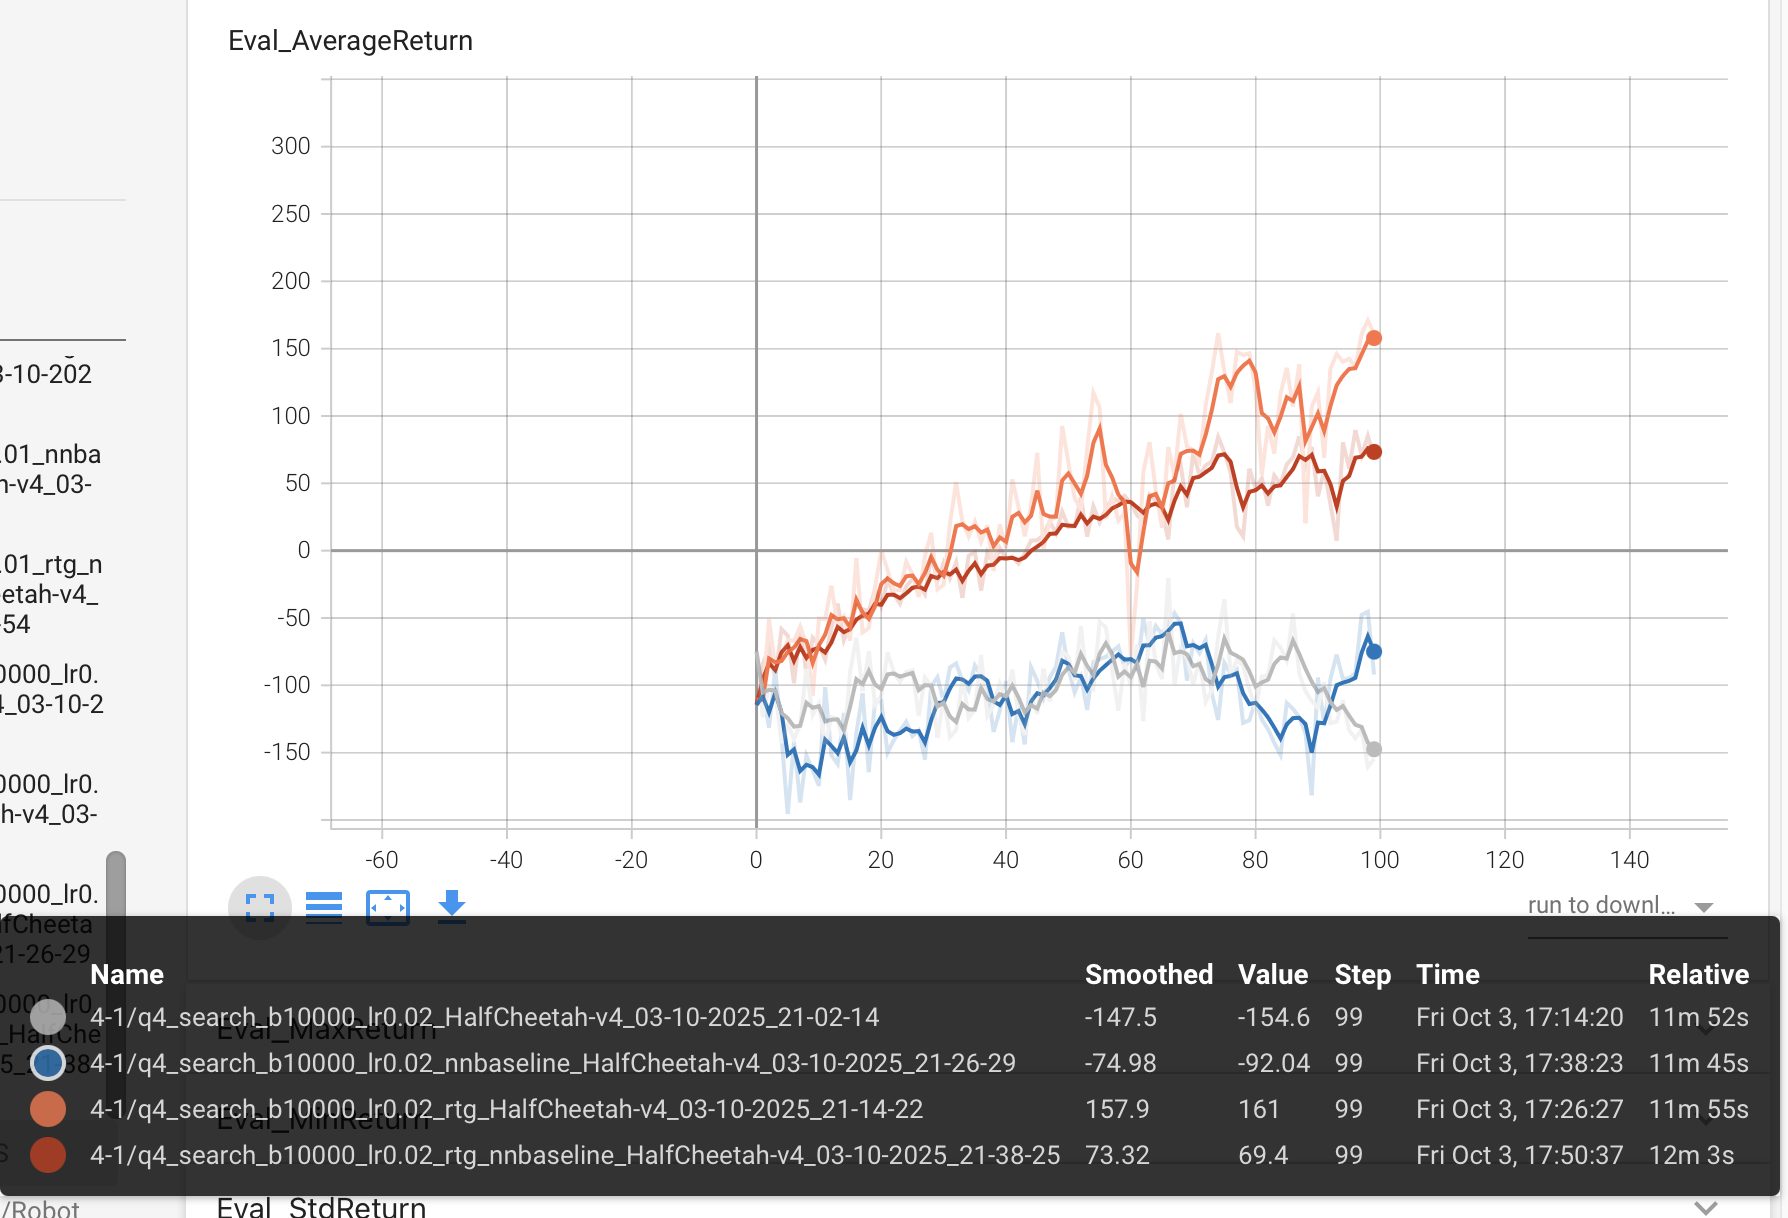
\includegraphics[height=8cm]{q4_1.png}
\end{answer}

\subsubsection{(bonus) Optimal b* and r* -- \lbrack0.5 points\rbrack}
\begin{answer}[title=Q7.2.3,height=4cm,width=\linewidth]
I found b*=35000, r*=0.01
\end{answer}

\subsubsection{(bonus) Plot -- \lbrack0.5 points\rbrack}
\begin{answer}[title=Q7.2.4,height=10cm,width=\linewidth]
\centering
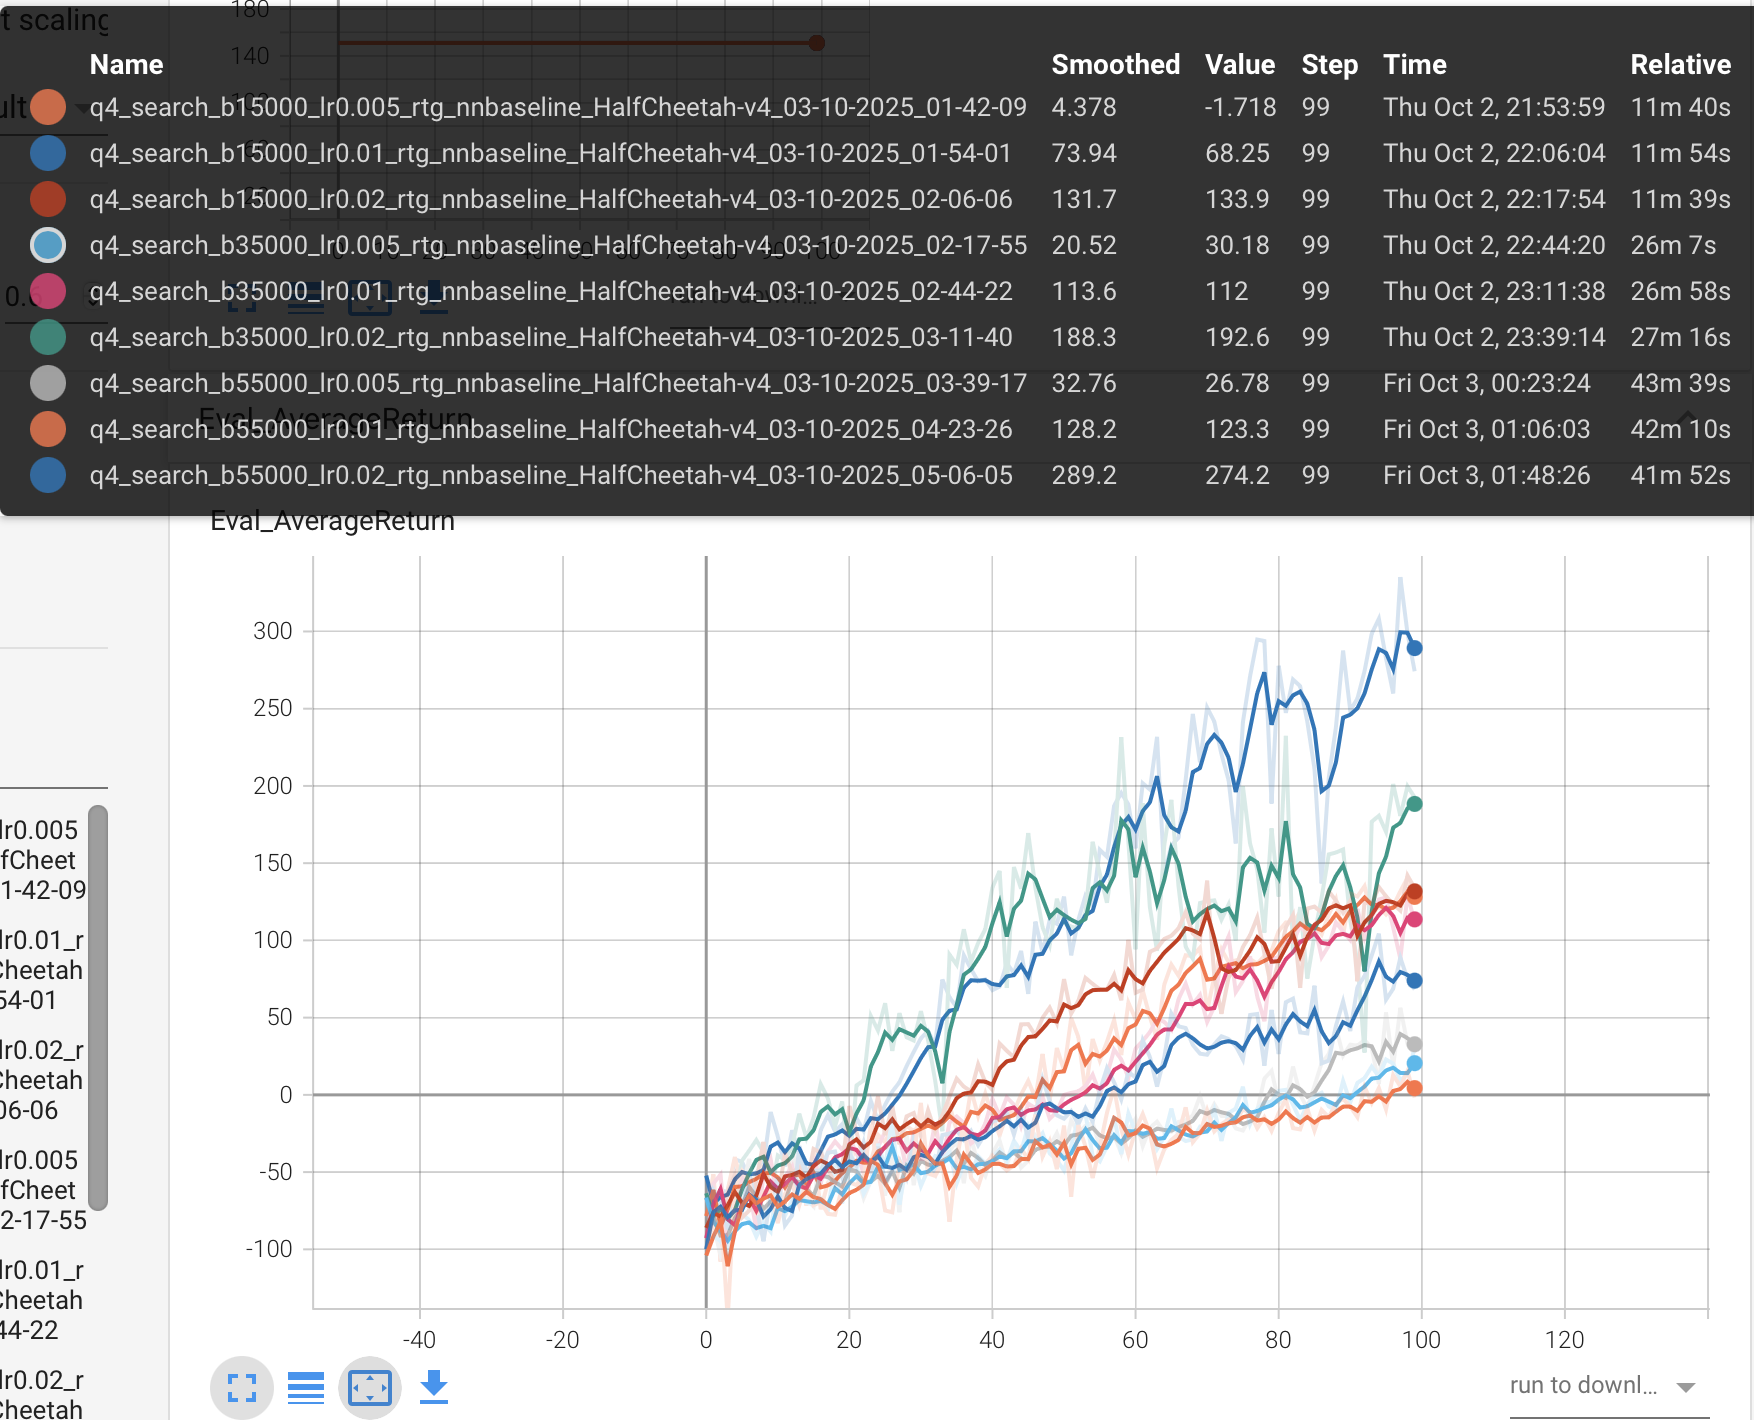
\includegraphics[height=8cm]{q4_2.png}
\end{answer}

\subsubsection{(bonus) Describe how b* and r* affect task performance -- \lbrack0.5 points\rbrack}
\begin{answer}[title=Q7.2.5,height=4cm,width=\linewidth]
Larger batches ($b=35\text{k}$–$55\text{k}$) produced smoother curves and faster, more reliable gains, while $b=15\text{k}$ was noticeably noisier and tended to plateau lower. The learning rate showed the usual bias–variance trade-off: $r=0.005$ was too conservative (slow improvement and lower final returns), whereas $r=0.02$ often became unstable with higher variance and occasional regressions. The mid-range $r=0.01$ consistently yielded the best performance and stability. Taken together, the results indicate an optimal setting around \boxed{b^=35{,}000,\ r^=0.01}, which balances sample efficiency and stable policy updates and attains the highest returns in the plot.
\end{answer}

\subsubsection{(bonus) Configurations with optimal b* and r* -- \lbrack0.5 points\rbrack}
\begin{answer}[title=Q7.2.6,height=6cm,width=\linewidth]
\begin{minted}
[framesep=2mm, fontsize=\scriptsize, breaklines]
{bash}
# Run HalfCheetah-v4 with b*=35000, r*=0.01

/content/py310/bin/python -m rob831.scripts.run_hw2 --env_name HalfCheetah-v4 --ep_len 150 \
  --discount 0.95 -n 100 -l 2 -s 32 -b 35000 -lr 0.01 --exp_name q4_b35000_r0.01

/content/py310/bin/python -m rob831.scripts.run_hw2 --env_name HalfCheetah-v4 --ep_len 150 \
  --discount 0.95 -n 100 -l 2 -s 32 -b 35000 -lr 0.01 -rtg --exp_name q4_b35000_r0.01_rtg

/content/py310/bin/python -m rob831.scripts.run_hw2 --env_name HalfCheetah-v4 --ep_len 150 \
  --discount 0.95 -n 100 -l 2 -s 32 -b 35000 -lr 0.01 --nn_baseline --exp_name q4_b35000_r0.01_nnbaseline

/content/py310/bin/python -m rob831.scripts.run_hw2 --env_name HalfCheetah-v4 --ep_len 150 \
  --discount 0.95 -n 100 -l 2 -s 32 -b 35000 -lr 0.01 -rtg --nn_baseline --exp_name q4_b35000_r0.01_rtg_nnbaseline
\end{minted}
\end{answer}

\subsubsection{(bonus) Plot for four runs with optimal b* and r* -- \lbrack0.5 points\rbrack}
\begin{answer}[title=Q7.2.7,height=10cm,width=\linewidth]
\centering
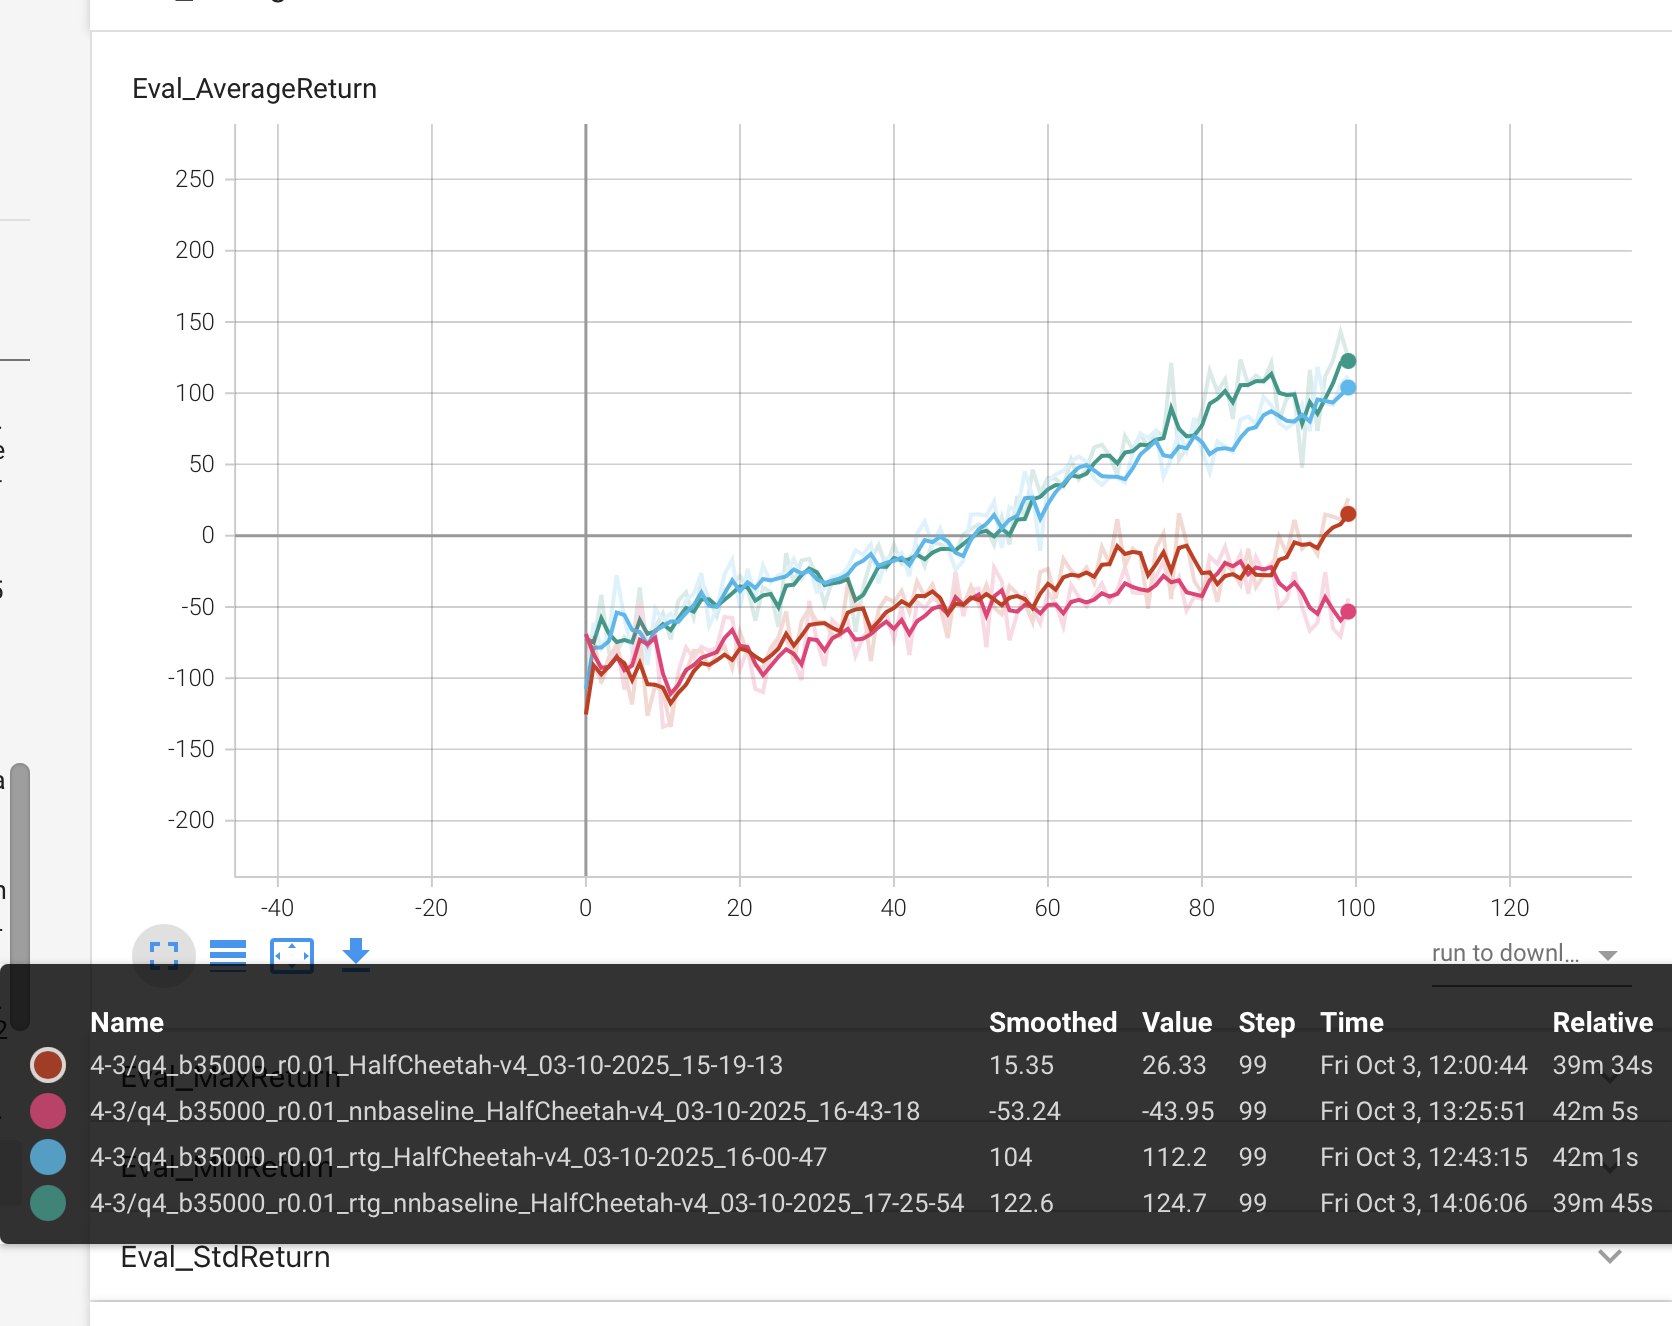
\includegraphics[height=8cm]{q4_3.png}
\end{answer}

\section{Implementing Generalized Advantage Estimation}

\subsection{Experiment 5 (Hopper) -- \lbrack4 points\rbrack}

\subsubsection{Configurations}
\begin{answer}[title=Q8.1.1,height=4cm,width=\linewidth]
\begin{minted}
[framesep=2mm, fontsize=\scriptsize, breaklines, escapeinside=||, mathescape=true]
{python}
# $\lambda \in [0,0.95,0.99,1]$
python rob831/scripts/run_hw2.py \
    --env_name Hopper-v4 --ep_len 1000
    --discount 0.99 -n 300 -l 2 -s 32 -b 2000 -lr 0.001 \
    --reward_to_go --nn_baseline --action_noise_std 0.5 --gae_lambda <|$\lambda$|> \
    --exp_name q5_b2000_r0.001_lambda<|$\lambda$|>
\end{minted}
\end{answer}

\subsubsection{Plot -- \lbrack2 points\rbrack}
\begin{answer}[title=Q8.1.2,height=10cm,width=\linewidth]
\centering
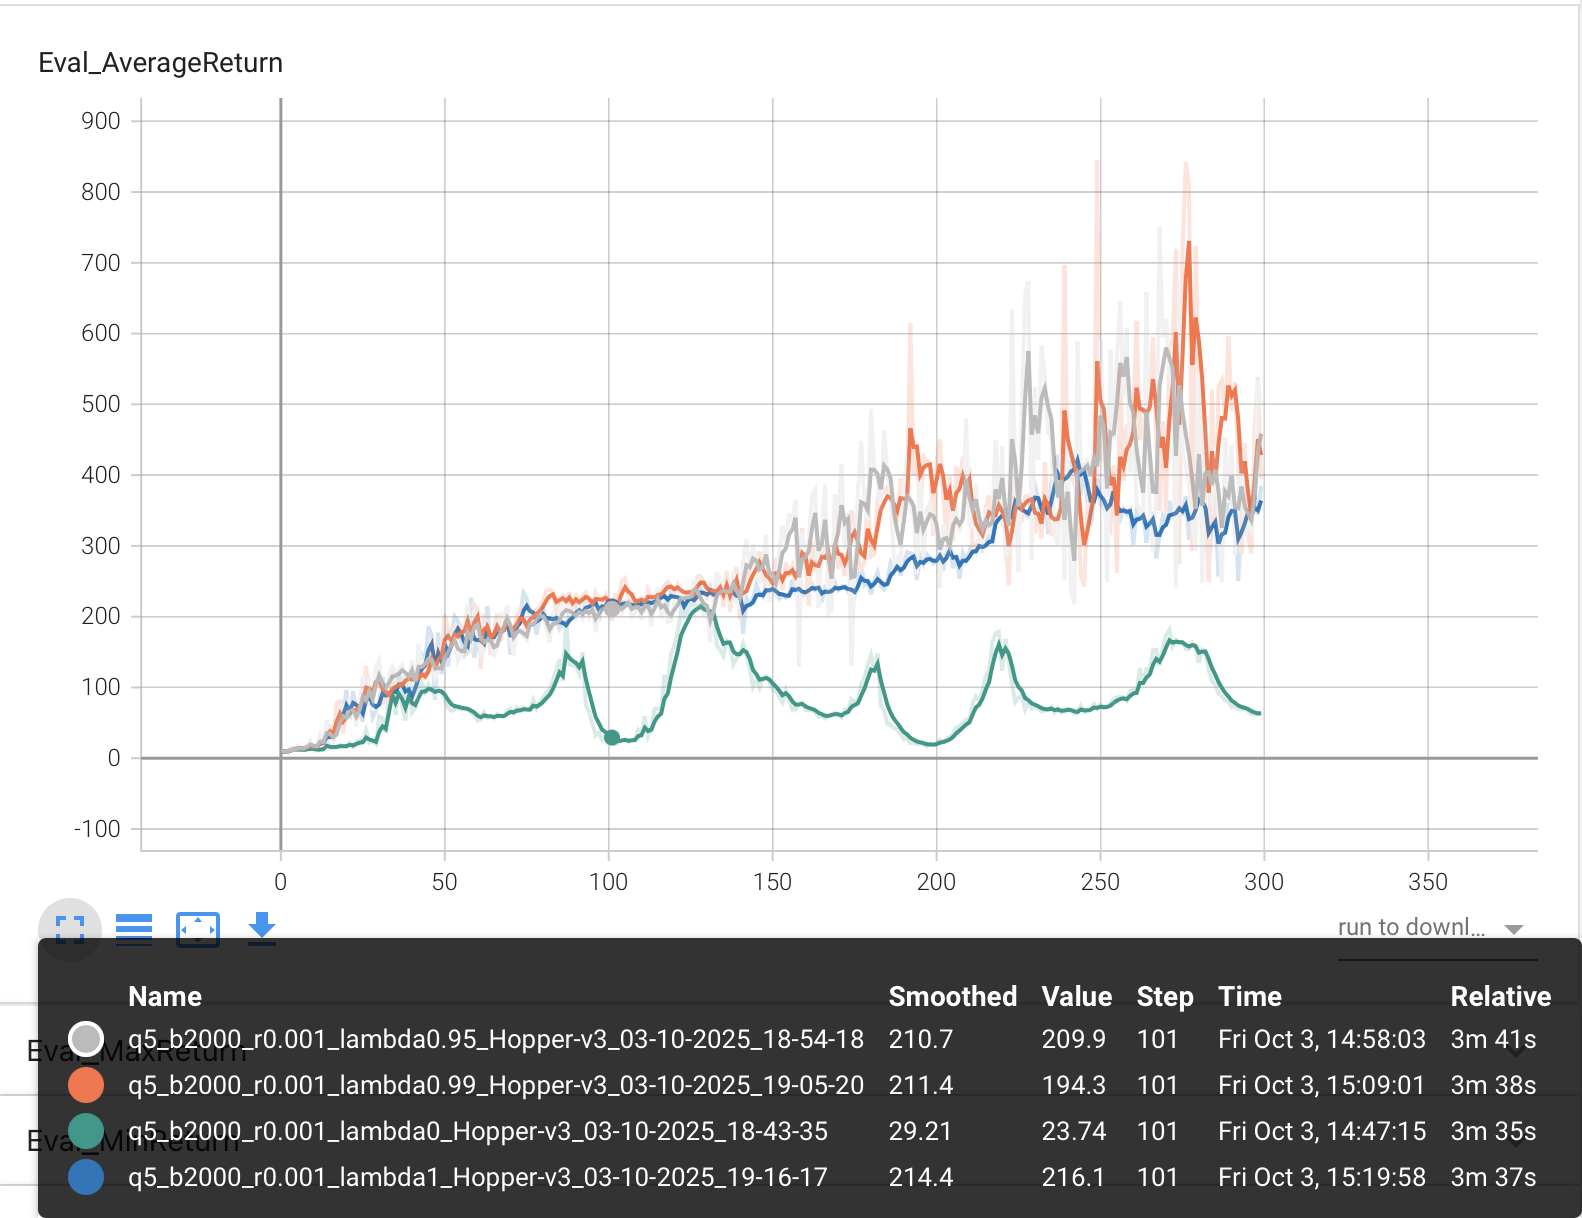
\includegraphics[height=8cm]{q5.png}
\end{answer}

\subsubsection{Describe how $\lambda$ affects task performance -- \lbrack2 points\rbrack}
\begin{answer}[title=Q8.1.3,height=4cm,width=\linewidth]
The choice of $\lambda$ strongly impacts both stability and final performance. At $\lambda=0$, the policy fails to learn effectively, oscillating with low returns below 250. Increasing $\lambda$ improves performance: $\lambda=0.95$ and $\lambda=0.99$ achieve the highest returns, with $\lambda=0.99$ reaching peaks above 600 but at the cost of higher variance and instability, while $\lambda=0.95$ provides steadier learning with returns in the 400–500 range. In contrast, $\lambda=1$ produces more stable but lower returns around 300–350, suggesting reduced variance but limited performance. Overall, moderate-to-high $\lambda$ values (0.95–0.99) strike the best balance between bias and variance, yielding faster learning and higher average returns compared to extreme values of $\lambda$.
\end{answer}

\clearpage

\section{More Bonus!}

\subsection{Parallelization -- \lbrack1.5 points\rbrack}
\begin{answer}[title=Q9.1,height=4cm,width=\linewidth]
% TODO (optional)
Difference in training time: 
\vspace{1.0cm}
\begin{minted}
[framesep=2mm, fontsize=\scriptsize, breaklines]
{bash}
python rob831/scripts/run_hw2.py \
\end{minted}
\end{answer}

\subsection{Multiple gradient steps -- \lbrack1 points\rbrack}
\begin{answer}[title=Q9.1,height=14cm,width=\linewidth]
% TODO (optional)
\centering
\includegraphics[height=8cm]{example-image-a}

\vspace{1.0cm}
\begin{minted}
[framesep=2mm, fontsize=\scriptsize, breaklines]
{bash}
python rob831/scripts/run_hw2.py \
\end{minted}

\end{answer}

\end{document}


